\chapter{Основное задание}

\section{Содержание проекта}

Команда разработчиков из 16 человек занимается созданием карты города на основе собственного модуля отображения. Проект должен быть завершен в течение 6 месяцев. Бюджет проекта: 50 000 рублей.

\section{Данные до начала выполнения заданий}

\textbf{Начало работ:} 01.03.2024. 

\textbf{Окончание работ:} 08.08.2024.

\textbf{Затраты:} 47 772 руб.

\textbf{Трудозатраты:} 9 261 ч.

\section{Содержание лабораторной работы}

Дата отчета: 17 мая.

Отметить как выполненные все работы, которые должны были завершиться на эту дату, кроме:

\begin{enumerate}
	\item Задача №5 фактически завершилась 22.03.
	\item С 18 марта программист №1 был направлен на стажировку, которая длилась 2 недели. В этот период его доступность в проекте составляла 30\%, продолжительность дня остальных программистов (№2-4) в это время составляла 9 часов. После обучения он был переведен на должность ведущего программиста («старого» ведущего программиста забрали в другой проект). Вся программистская работа перераспределилась между программистами №2-4, их зарплата с этого момента выросла на 20\%, а рабочий день опять стал 8-часовым.
	\item С 8 апреля на 10\% была увеличена зарплата мультимедиа-корреспондента.
	\item Задача №17 выполнена на 60\%.
	\item 1 апреля для задачи «Создание мультимедиа наполнения» купили специализированное ПО стоимостью 500 рублей и еще 100 рублей понадобилось на его установку.
	\item С 1 апреля заключили договор с партнерской организацией, что позволило отказаться от арендованного сервера, так как организация предоставила свой сервер на безвозмездной основе. Помимо этого, договор предусматривает оказание организацией – партнером сервисных услуг на сумму 3200 рублей до конца проекта.
\end{enumerate}

\section{Задание 1: Актуализация параметров проекта}

Была задана дата отчета по заданию: 17 мая.

\begin{figure}[H]
    \begin{center}
    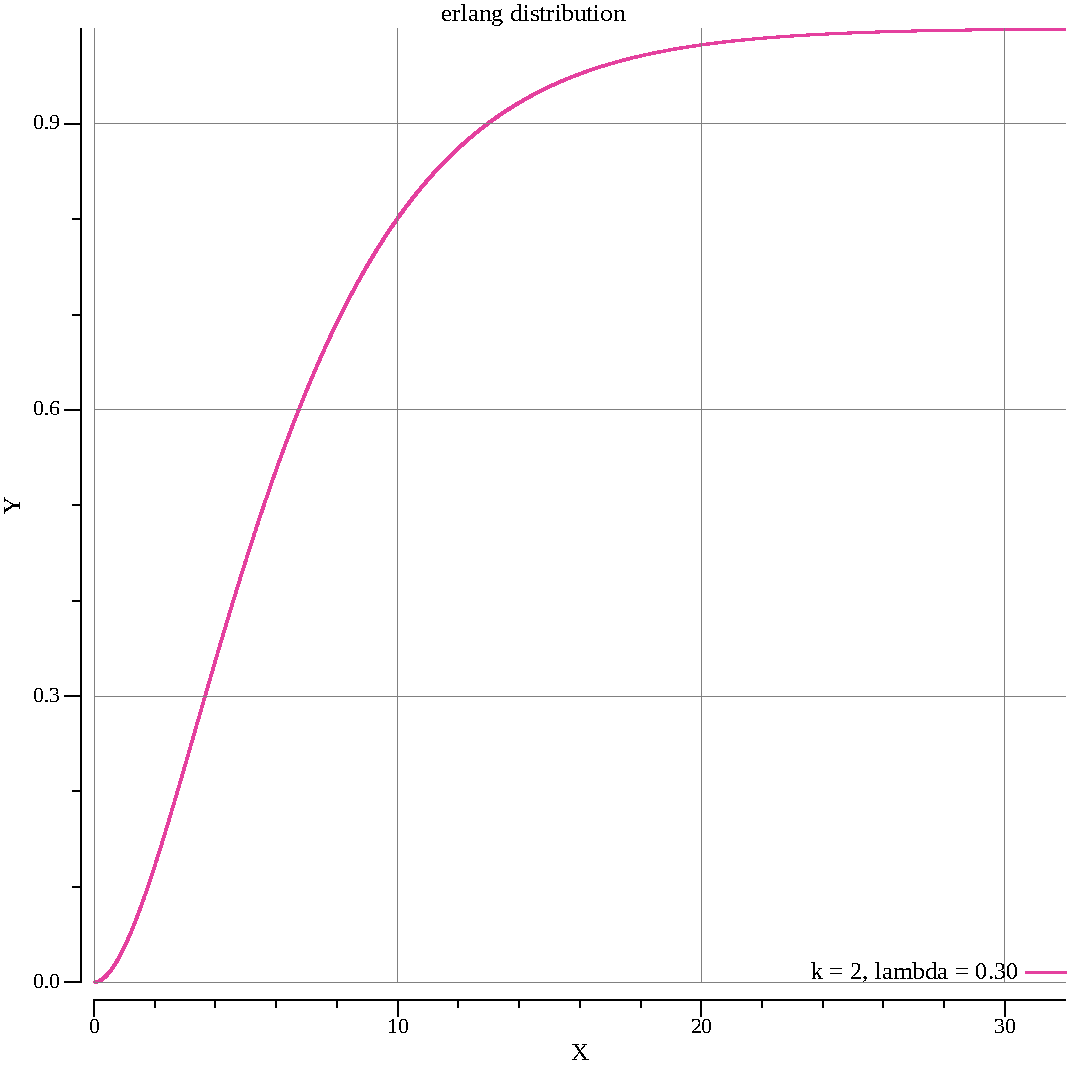
\includegraphics[width=0.5\linewidth]{assets/1}
    \caption{Задание даты отчета}
    \label{fig:1}
    \end{center}
\end{figure}

Была установлена фактическая дата завершения задачи 5: 22 марта.

\begin{figure}[H]
    \begin{center}
    
\includegraphics[width=1\linewidth]{assets/2}
    \caption{Изменение фактической даты завершения задачи 5}
    \label{fig:2}
    \end{center}
\end{figure}

Из-за стажировки программиста 1 были внесены изменения в графики работ и доступность ресурсов. Доступность программиста 1 на время с 18 марта по 31 марта составляла 30 процентов.

\begin{figure}[H]
    \begin{center}
    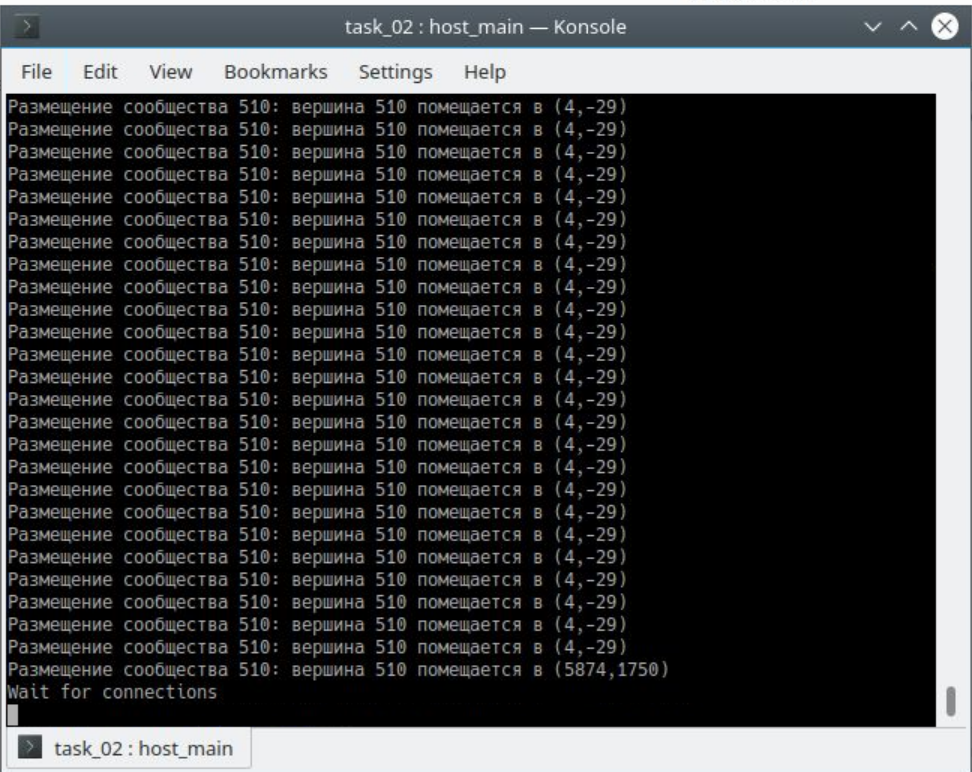
\includegraphics[width=1\linewidth]{assets/3}
    \caption{Изменение доступности программиста 1}
    \label{fig:3}
    \end{center}
\end{figure}

Рабочий день программистов 2-4 составлял 9 часов на этот период.

\begin{figure}[H]
    \begin{center}
    \includegraphics[width=1\linewidth]{assets/4}
    \caption{Изменение рабочего времени программистов 2-4}
    \label{fig:4}
    \end{center}
\end{figure}

После окончания стажировки (с 1 апреля) программист 1 был переведен на должность ведущего программиста, с соотвествующим повышением зарплаты.

\begin{figure}[H]
    \begin{center}
    \includegraphics[width=1\linewidth]{assets/5}
    \caption{Повышение зарплаты программиста 1}
    \label{fig:5}
    \end{center}
\end{figure}

После возвращения программиста 1, зарплаты остальных программистов выросли на 20 процентов.

\begin{figure}[H]
    \begin{center}
    \includegraphics[width=1\linewidth]{assets/6}
    \caption{Повышение зарплаты программистов 2-4}
    \label{fig:6}
    \end{center}
\end{figure}

После возвращения программиста 1, старого ведущего программиста забрали в другой проект, и его роль исполняет программист 1. Таким образом, доступность ведущего стала 0, его сняли с задач.

\begin{figure}[H]
    \begin{center}
    \includegraphics[width=1\linewidth]{assets/7}
    \caption{Программист 1 назначен вместо ведущего}
    \label{fig:7}
    \end{center}
\end{figure}

С 8 апреля на 10 процентов была повышена зарплата мультимедиа-корреспондента.

\begin{figure}[H]
    \begin{center}
    \includegraphics[width=1\linewidth]{assets/8}
    \caption{Повышение зарплаты мультимедиа-корреспондента}
    \label{fig:8}
    \end{center}
\end{figure}

Задача 17 выполнена на 60 процентов.

\begin{figure}[H]
    \begin{center}
    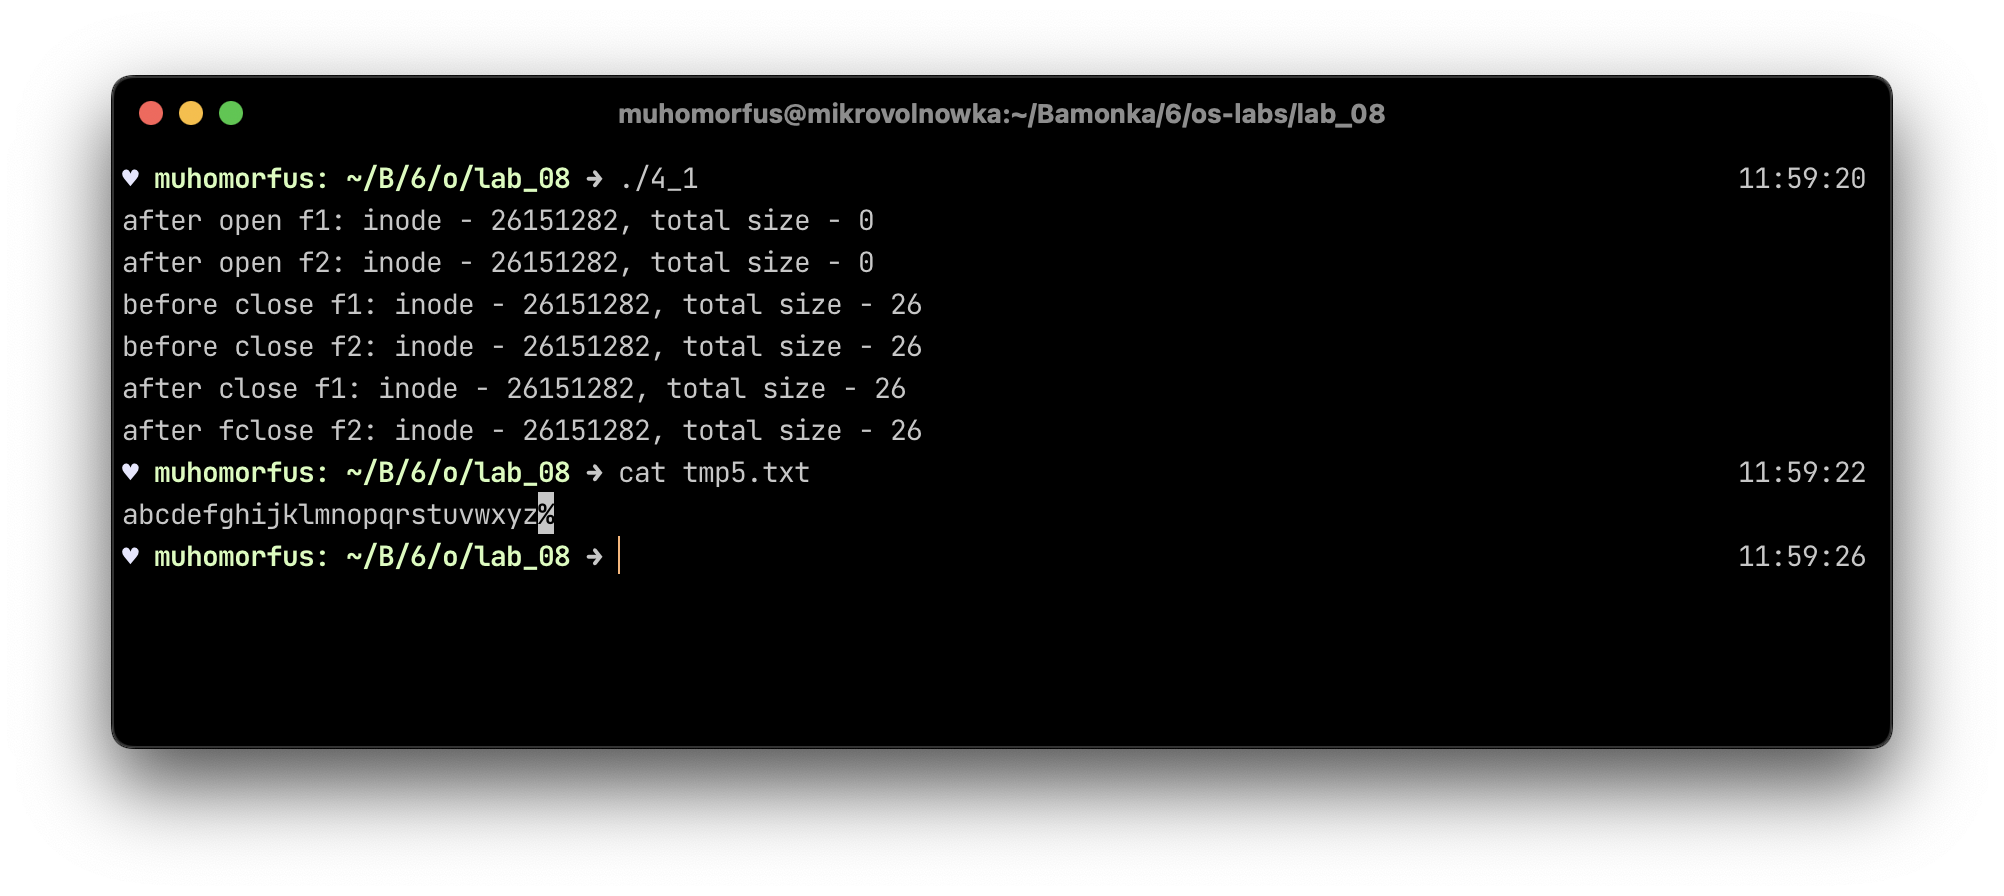
\includegraphics[width=1\linewidth]{assets/9}
    \caption{Задача 17 выполнена на 60 процентов}
    \label{fig:9}
    \end{center}
\end{figure}

1 апреля для задачи «Создание мультимедиа наполнения» купили специализированное ПО стоимостью 500 рублей и еще 100 рублей понадобилось на его установку. Соответственно, был создан материальный ресурс ПО стоимостью 500 рублей и с фиксированными затратами 100 рублей. Ресурс был назначен на задачу.

\begin{figure}[H]
    \begin{center}
    \includegraphics[width=1\linewidth]{assets/10}
    \caption{ПО}
    \label{fig:10}
    \end{center}
\end{figure}

С 1 апреля заключили договор с партнерской организацией, что позволило отказаться от арендованного сервера, так как организация предоставила свой сервер на безвозмездной основе. Помимо этого, договор предусматривает оказание организацией – партнером сервисных услуг на сумму 3200 рублей до конца проекта. Были назначены фиксированные затраты на целевую задачу проекта в 3200 рублей.

Сервер был настроен так, чтобы оплата по нему шла до 1 апреля.

\begin{figure}[H]
    \begin{center}
    \includegraphics[width=1\linewidth]{assets/12}
    \caption{Оплата сервера}
    \label{fig:12}
    \end{center}
\end{figure}

На экран была выведена линия прогресса.

\begin{figure}[H]
    \begin{center}
    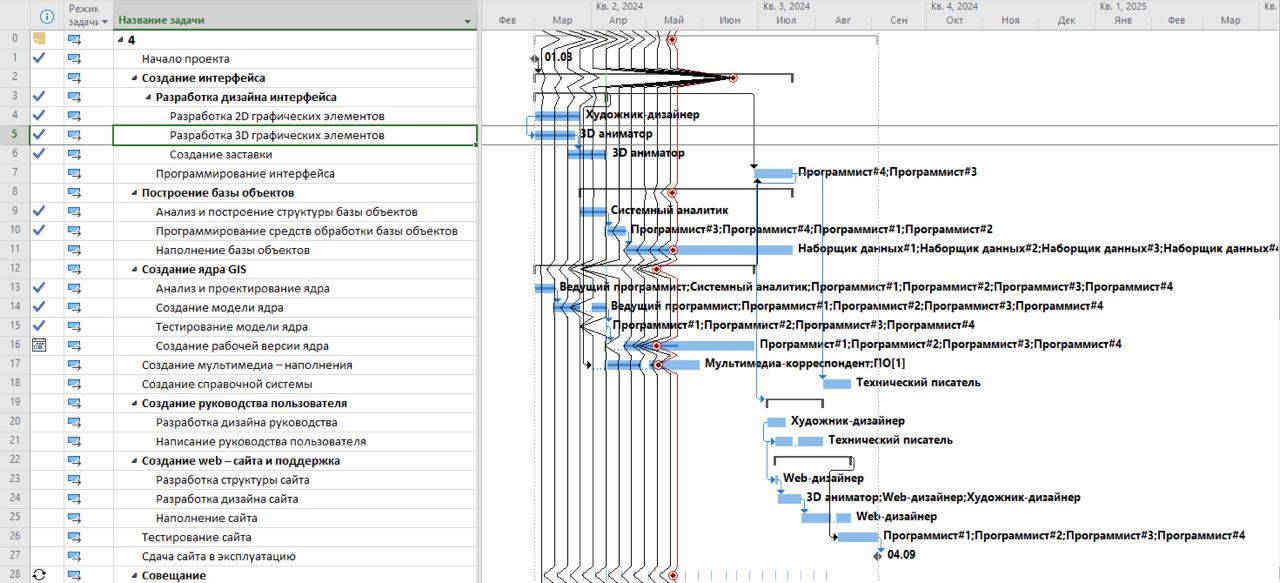
\includegraphics[width=1\linewidth]{assets/13}
    \caption{Линия прогресса}
    \label{fig:13}
    \end{center}
\end{figure}

На основании анализа линий выполнения можно сделать следующие выводы.

\begin{enumerate}
	\item Задача 17 (создание мультимедиа наполнения) на дату отчета выполнялась быстрее запланированного.
	\item Задачи, связанные с созданием ядра GIS сильно отстают от графика. Это связано с уходом ведущего программиста и частичной недоступностью программиста 1 в течение двух недель.
	\item Задачи, связанные с созданием интерфейса опережают план, так как задача 5 фактически завершилась раньше.
\end{enumerate}

Статистика по проекту:

\begin{figure}[H]
    \begin{center}
    \includegraphics[width=1\linewidth]{assets/14}
    \caption{Статистика по проекту}
    \label{fig:14}
    \end{center}
\end{figure}

В результате актуализации проекта стоимость изменилась с 47772 рублей до 49138 рублей. Дата окончания проекта изменилась с 8 августа до 13 августа. Для улучшения показателей проекта возможно имело бы смысл нанять еще одного программиста вместо ушедшего ведущего, перед уходом первого программиста на стажировку.
